\section{Implementação}

Definida uma estrutura base para a arquitetura do projeto,
determinando-se como cada parte da estrutura construída ia ser
implementada na solução final.

\subsection{Ficheiros .3d}

Tomou-se como ponto de partida a definição da estrutura dos ficheiros que
vão ser usados para comunicação das primitivas entre o gerador e o motor
gráfico.\newline
\break
\noindent
Decidiu-se, portanto, por questões de facilidade e eficiência de leitura
e escrita, usar uma solução binária para a composição destes
ficheiros.\newline
\break
\noindent
Cada ponto deverá escrever as suas coordenadas em formato de
\textit{float} binário, ocupando no ficheiro 4 bytes por
valor de coordenada, ou, na totalidade, 12 bytes pelas três
coordenadas x, y, z de cada ponto.\newline
\break
\noindent
Cada três pontos definirão uma face, originando um custo de 36 bytes
por face, e um conjunto de faces representarão uma primitiva,
produzindo um custo de NrFaces * 36 bytes por ficheiro.\newline
\break
\noindent
Em ficheiro, este formato pode, portanto, ser visto, considerando
os espaços e os parágrados como inexistentes, da seguinte forma:\newline

\begin{tcolorbox}[
    colback=gray!10!white,
    colframe=black!50!black,
    after upper={\hfill\textbf{.3d simplificado}}
]
\begin{verbatim}
0.0000 0.0000 0.0000 (em binário) | Face1
...Ponto2...                      | Face1
...Ponto3...                      | Face1
...Ponto4...                      | Face2
...Ponto5...                      | Face2
...Ponto6...                      | Face2
...Ponto7...                      | Face3
...                               ...
\end{verbatim}
\end{tcolorbox}

\break
\noindent
Embora não seja o principal motivo, esta estrutura binária também irá
permitir uma redução do espaço que estes ficheiros ocuparão no disco em
comparação a uma solução baseada num formato textual.\newline

\subsection{Gerador de Primitivas}

Estipulado o formato dos ficheiros que deverão ser usados para armazenar
e representar primitivas, é necessário definir como o gerador irá criar e
guardar estes modelos de acordo com a estrutura decidida.\newline
\break
\noindent
Para a sua implementação, foi decidido usar uma abordagem por matrizes
para a representação dos pontos, aproveitando a eficiência de cálculo
que estas trazem para a aplicação de transformações aos pontos que irão
constituir as primitivas.\newline
\break
\noindent
Como deliberado na conceptualização, o gerador será composto por uma
hierarquia de primitivas que contêm faces, que, por sua vez, contêm
pontos. Esta arquitetura trará bastantes vantagens para a construção
de modelos, permitindo aplicar transformações a vários pontos que estejam
contidos numa face (ou numa primitiva) de uma só vez.\newline
\break
\noindent
Este conceito permite a possibilidade de ver as primitivas como uma
espécie de conjunto de sub-primitivas que se repetem ao longo do modelo
com diferentes posições e rotações.\newline
\break
\noindent
Assim sendo, é possível criar uma primitiva através de várias cópias
de uma ou mais sub-primitivas aplicando-lhes diferentes translações
e rotações de forma a obter um modelo definitivo final.\newline
\break
\noindent
Esta estratégia permitirá, então, a criação de primitivas através de
uma simples inicialização de elementos comuns na estrutura e posterior
aplicação de diferentes transformações a várias cópias destes, evitando
a criação singular de cada ponto necessária à representação final
da figura tridimensional.\newline
\break
\noindent
Ainda se decidiu implementar métodos de auxilio à criação destas
matrizes de translação, rotação e pontos, existindo a hipótese de
gerar pontos e translações através de coordenadas polares, que serão
bastante úteis para a representação do cone, por exemplo.

\subsection{Primitivas}

Aproveitando o conceito definido anteriormente para a definição de
primitivas, definiu-se, de forma simples, como poderiam os modelos
pretendidos ser, então, gerados.

\subsubsection{Plano}

Usando como ponto de partido o modelo mais simples (e que virá auxiliar
na criação de um outro modelo), o processo de definição deste começa pela
perceção do plano como um conjunto de planos mais pequenos, no caso de
as divisões pretendidas serem superior a uma.\newline
\break
\noindent
Esta visão permite, portanto, definir o plano como a criação
de um primeiro quadrado (o da sub-divisão de um canto, por exemplo)
e da translação de várias cópias deste quadrado de forma a obter um
quadrado maior constituído por menores quadrados.\newline
\break
\noindent
Esta transformação pode ser feita construíndo, no ínicio, uma linha
inferior de quadrados e multiplicando-o para cima, como pode ser visto
na Figura \ref{fig:plane}.

\begin{center}
    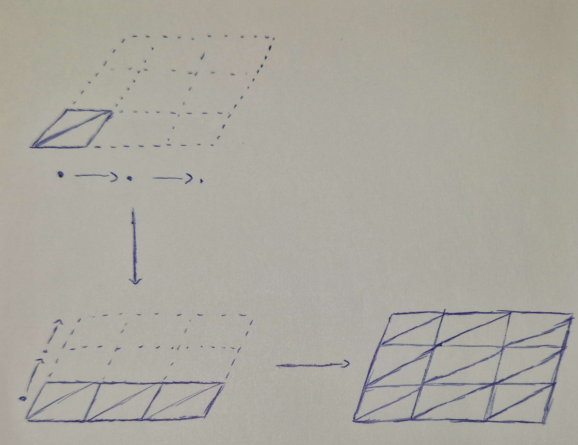
\includegraphics[width=0.6\textwidth]{imgs/plane.png}
    \captionof{figure}{Construção do plano}
    \label{fig:plane}
\end{center}

\subsubsection{Caixa}

Considerando o modelo da caixa, é rapidamente percétivel que esta pode ser
definida através de seis planos, aplicando-lhes rotações e translações.\newline
\break
\noindent
Esta definição torna-se, portanto, extremamente simples devido à já
existência de uma definição para plano, podendo ser definida pelas
transformações necessárias à criação da face superior e inferior e
posterior rotação de ambas para a criação das faces restantes.

\begin{center}
    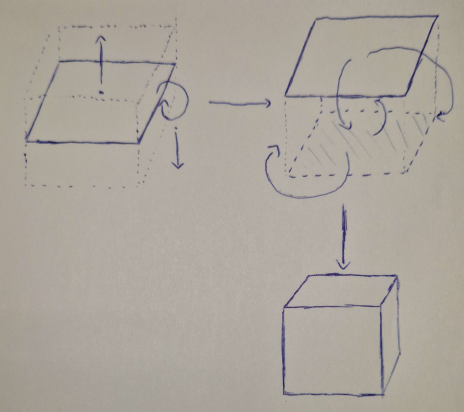
\includegraphics[width=0.6\textwidth]{imgs/box.png}
    \captionof{figure}{Construção da caixa}
    \label{fig:box}
\end{center}

\subsubsection{Esfera}

Focando num modelo mais complexo, a esfera será mais complicada de
definir devido à sua curvatura, porém ainda será possível aproveitar
conceitos vistos anteriormente.\newline
\break
\noindent
A ideia da definição da esfera começa na perceção da mesma como várias
fatias iguais, dividas sobre o eixo y. Esta percepção permitirá,
simplesmente, duplicar a primeira fatia através de rotações
pelo eixo y de forma a obter várias iguais, deixando o desafio
apenas na definição da primeira fatia.\newline
\break
\noindent
Será necessário, então, pensar na fatia como dois arcos de pontos que
se ligam através de triângulos ou quadrados, em que um arco pode ser
obtido através do outro com uma simples rotação sobre o eixo y.\newline
\break
\noindent
Fica necessário apenas definir um arco. Este pode ser visto, portanto,
como várias rotações de um ponto sobre o eixo x até fazer
meia rotação completa ao eixo.\newline
\break
\noindent
Este processo pode, portanto, ser visualizado na Figura \ref{fig:sphere}.

\begin{center}
    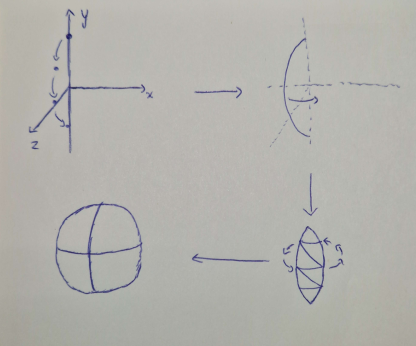
\includegraphics[width=0.6\textwidth]{imgs/sphere.png}
    \captionof{figure}{Construção da esfera}
    \label{fig:sphere}
\end{center}

\subsubsection{Cone}

Por último, sendo algo também complicado, apenas é necessário definir o
cone, que adotará uma estratégia semelhante à da esfera, dividindo em
fatias.\newline
\break
\noindent
O problema encontra-se, mais uma vez, na definição da primeira fatia
onde poderá ser usada, também, uma abordagem semelhante à da esfera,
divisão em dois triângulos que podem ser obtidos por uma rotação.\newline
\break
\noindent
O primeiro triângulo será, então, simples de obter, sendo apenas
necessário aplicar sucessivas translações polares (com um ângulo a 
apontar para o topo do cone) ao ponto da base do cone até este atingir
o topo desejado.\newline
\break

\begin{center}
    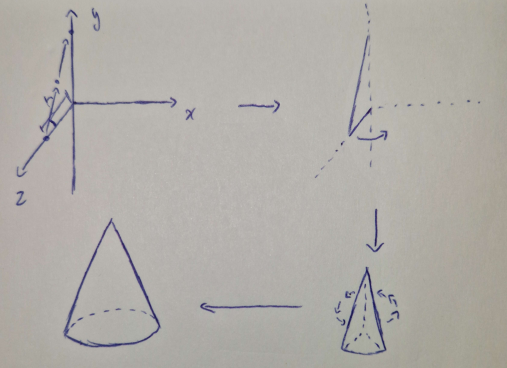
\includegraphics[width=0.6\textwidth]{imgs/cone.png}
    \captionof{figure}{Construção do cone}
    \label{fig:cone}
\end{center}

\subsection{Motor Gráfico}

Estruturada e decidida a implementação do gerador de primitivas, existe,
ainda, a necessidade de definir como estas vão ser lidas, armazenadas e
representadas no motor gráfico.\newline
\break
\noindent
Não existindo a exigência de realizar translações, rotações, etc. à
estrutura dos modelos (ainda poderão ser realizadas transformações às suas
representações), decidiu-se definir os pontos como três \textit{float},
em constraste à abordagem matricial seguida anteriormente, devido à
necessidade única do armazenamento das propriedades.\newline
\break
\noindent
Assim sendo, o motor gráfico apenas recorrerá à utilização de métodos para
a leitura dos ficheiros definidos para o armazenamento, para a leitura dos
ficheiros \textit{XML} que definem as propriedades de um cenário
e para a representação deste cenário e das suas primitivas
através das funcionalidades ofericidas pelo
\textbf{OpenGL} e \textbf{GLUT}.\newline
\break
\noindent
Estes métodos serão, ainda, definidos de acordo com a hierarquia
já definida na conceptualização, sendo que cada objeto ficará
encarregue da sua interpretação em ficheiro, quer seja \textit{XML}
ou \textit{3d}.